\chapter{Financialization} \label{chapter-financialization}

*** ADD MORE ON THE LITERATURE ON FINANCIALIZATION TO SETUP OUR WORK, AS IN THE ABOVE CHAPTERS

%BASED ON Financialization_of_the_Housing_Market.tex
Financialization is %the process by which financial institutions, markets, etc., increase in size and influence. More specifically it is
the process by which future streams of revenue and speculative gains are 
 %systematically 
captured by individuals and institutions with financial assets. %\footnote{In the industry it is more common to describe financialzation as creating ownership instruments that allow streams of income to be traded by investors. The emphasis is on enabling investors to participate.} 
It may be understood as the process by which which financial institutions, markets, etc., increase in size and influence. 

Financialization of the housing market is the increasing control of the stock of urban land and housing in order to capture the scarcity rent generated by the people of the city.  Mortgages and REITs are both financial instruments.
% \section{Literature on theory and evidence} % PROVIDE EVIDENCE 	mention theories?
There is substantial evidence that the financialization of urban housing is underway in Canadian cities..

Two questions arise when we observe the growing participation of global capital in the urban housing system: 
\begin{enumerate}
\item How far will the financialization of urban land go? 
\item That are the implications for the urban economy and the welfare of the urban population? 
\end{enumerate}

We can demonstrate that in the absence of policy interventions, differential access to finance capital ensures that capital owners acquire an increasing share of urban land % over time
and therefore capture the growing land rents from urban productivity growth. 

With this insight, growing wealth inequality emerges within a simple, widely accepted model of the urban land market. In the limit, urban residents are tenants, and new residents without capital no longer receive any of the increases in rents arising from the growing productivity of the city. 

%The first question, therefore, is reduced to which capital holders will increase their share of urban land and whether there is any reason to expect the process of financialization process to stop or reverse itself.

% \section{The incentives for financialization}%\label{Sec:RentAndClass}
%Instead, drawing on the ideas of Jane Jacobs, Lucas proposes the city as the unit of analysis. Lucas, Robert (1990), "Why Doesn't Capital Flow from Rich to Poor Countries?," American Economic Review Papers and Proceedings v. 80, no. 2 (May) pp. 92-96.  
%Jacobs, Jane  (1969), The Economy of Cities (New York: Random House).  
% The Death and Life of Great American Cities \cite{Jacobs61}



\section{The rate of return on a property purchase}
% ADD TABLE WITH VARIABLE DEFINITIONS


 
 In this section we model the return on an investment in urban properties. We model agents as %'ll assume that all agents are
 speculating on potential \glspl{capital gain} as well as on the \gls{use value} they get from living in a property. %We assume that the use value is captured by the stream of rental values. %, whether a home is owner-occupied or held by an investor as a financial asset. 
 % For simplicity, we consider a one-period investment.  %To keep the analysis simple without loss of generality 

 The agent purchases a house for a price, $P_0$ %a down payment, $D$, 
 and receives the increased price $P_T = (1 + \dot P)P_0$, back after a period $T$. 
% The value of the investment is the net present value of buying and then selling after one period:
The value of the investment is the capital gain, $\mathcal{C}$ plus the rents, net of operating costs and taxes, $\mathcal{R}_N$.

% minus the mortgage, repaid with interest, plus rents, minus any operating costs and taxes,\footnote{We have applied this model to explore the effect of a vacancy tax in Beirut.  For that analysis we  added a use-value, $U$ in place of rent for expatriate owners to represent using the property - say one month a year - when they are not renting the property and a \textbf{vacancy tax}, $T$ at rate $t$ to affect the speculator's  decision.} %\cite{Al-Shihabi}

\begin{eqnarray}
V &=& \mathcal{C} + \mathcal{R}_N \nonumber \\
  &=& \mathcal{C} + \mathcal{R} - \mathcal{O} - \mathcal{T} \nonumber \\
  &=& \delta \left(P_T- \left(1+r\right)M\right) + \mathcal{R} - \mathcal{O} - \mathcal{T}. \label{Eqn:V1}
\end{eqnarray}

% OLD equations from working out the above. Could change symbols
% \begin{eqnarray}
% V  	&=& capital\ gain - Interest\ due  	+ Rent  - operating\ cost -taxes\\
% 	&=& \delta P_T-D \qquad \qquad \quad - (1+\delta r)M \quad	 + R  	-C\\
% 	&=& \delta P _T \qquad-(P_0-M) \quad- (1+\delta r)M 	 + R  	-C\\
% 	&=& \delta (1+\dot P)  P_0 -(P_O -M)  -(1+\delta r)mP_0  + R  -C\\
% 	&=& \delta (1+\dot P)  P_0 -P_O + M \qquad -(1+\delta r)mP_0  + R -C\\
% 	&=&( \delta (1+\dot P)-1)  P_0  + mP_0 \quad -(1+ \delta r)mP_0  + (\rho-\kappa)P_0\\	
% 	&=& \left(  \delta (1+\dot P)-1    + m \quad - m(1+\delta r)  + (\rho-\kappa)\right)P_0\\'
% 	&=& \left(  \delta (1+\dot P)-1    + m \quad - m-\delta rm  + (\rho-\kappa)\right)P_0
% \end{eqnarray}

 Where $\mathcal{R}$, $\mathcal{O}$, $\mathcal{T}$, and $M$ are  net present values for rent, operating costs, tax payments, and the mortgage at the end of the period. The interest rate is $r$, and the discount factor $\delta$.

 For ease of calculation, this may also be written in terms of shares of the purchase price:

 \begin{eqnarray}
  V &=& \delta \left((1+\dot P) P_0 - (1+r)mP_0\right) + \rho P_0 - \theta P_0 - \tau P_0 \nonumber \\
    &=& \left(\delta \left(1+\dot P - (1+r)m   \right) + \rho     - \theta     - \tau\right) P_0. \label{Eqn:V2}
 \end{eqnarray}
 
 Where $\rho$, $\theta$, $\tau$, and $m$ are rent, operating costs, taxes, and mortgage shares. 
 % of price for rents, operating costs, and taxes. %The discount factor is $delta$, $P_0$ is the property price at the time of sale. %$r$ is the interest rate paid, and $m$ is the share of the price taken out as a mortgage.
 %It has  seven  parameters, $\delta, \dot P, r, m, \rho, \kappa$ and $t$. The first four, $\delta, \dot P, r$ and $m$ are exogenous for the investor while $\rho$, $\kappa$ and $t$  are    %Operating revenue and costs $\rho, \kappa$ and $t$ are expressed as  present values. 
 
 MOVE The mortgage share and interest rate are functions of the agents wealth %Both the  share of the price  that can be mortgaged, $m$, and the interest rate and the interest rate paid, $r$, are functions of the agent's wealth. 
The discounting factor may be correlated with wealth as well. 

The rate of return on funds invested, $r_{return}$, is the value divided by the size of the downpayment, $D$: 
%The rate of return is $v = \frac{V}{D}$. %For expat investors, we get a \textbf{decision rule}:
%\begin{enumerate}
%\item  if $v \geq a$ (with some private use?) with no rent,  don't bother renting. 
%\item If $v(no\ rent\ and\ tax) < a\geq v(with\ rent)$,  then  rent. 
%\item If $ v(with\ rent) \le a $,  then sell 
%\end{enumerate}\
\begin{eqnarray}
r_{return} 
 &=& \frac{V}{D}  \nonumber \\
 &=& \left(\delta \left(1+\dot P - (1+r)m\right) \ + \rho - \theta - \tau \right) \frac{P_0}{D}        \nonumber \\
 &=& \left(\delta \left(1+\dot P - (1+r)m\right) \ + \rho - \theta - \tau \right) \frac{P_0}{P_0-mP_0} \nonumber \\ 
 &=& \frac{\delta \left(1+\dot P - (1+r)m\right) \ + \rho - \theta - \tau }{1-m}. \label{Eqn:DecisionRule2}
\end{eqnarray}
Equation~\ref{Eqn:DecisionRule2} provides a criterion for investors. Agents invest if if their expected return is greater than the target return, they are seeking:
\begin{equation}
r_{return} \geq r_{target}.
\end{equation}
The rule has long run implications for the ownership of housing. 

%The implications of {\color{red} Equation~\ref{Eqn:DecisionRule2}} are significant for the evolution of the urban land market and class structure.  
Some of the implications include:

\begin{enumerate}
\item A large $m$ magnifies the return. (The downpayment is smaller as a fraction of the price, increasing the investor's leverage). 

\item A lower mortgage interest rate increases the return by lowering interest payments.  The wealthy can generally borrow  at lower interest rates than the less wealthy. 

\item A lower discount rate $\delta$ reduces the subjective rate of return.  \footnote{Poverty in assets, or cash liquidity constraints, was leading to or correlated with higher rates of time preference. Poverty, market imperfections and time preferences: of relevance for environmental policy?   S. Holden, B. Shiferaw, M. Wik.  1998, Environment and Development Economics https://www.semanticscholar.org/paper/Poverty %2C-market-imperfections-and-time-preferences%3A-Holden-Shiferaw/55376ceb29b6f3bab2d8fb3dd83d5904826959ac
}
\item Higher expected price appreciation increases the attractiveness of investment. The wealthy and financial corporations  are likely to have better price forecasts than  the occasional home buyer.
\item Higher rents make the unit more profitable. higher expected  rents may result from expecting greater price appreciation raises expected profitability or greater willingness to raise rents for tenants 

\item Lower maintenance costs increase profits. There may be scale economies in the maintenance  of rented housing. 
\item Lower tax rates decrease holding costs and increase the value of the investment. here may be opportunities to shelter income with land held for investment (speculative) purposes
\end{enumerate}
%As expected
%\begin{enumerate}
%\item A large $m$ magnifies the return. (downpayment is smaller)
%\item A lower mortgage interest rate increases the return because of interest on the mortgage
%\item A lower discount rate $\delta$ reduces the subjective rate of return
%\item Higher expected price appreciation increases the attractiveness of investment
%\item Higher rents makes the unit more profitable if rents are being collected
%\item Lower costs increase profits
%\item Lower tax rates decrease holding costs and increase the value of the investment
%\end{enumerate}

Since interest rates are lower for those with higher wealth, it implies, consistent with the empirical evidence, that net returns for investment are increasing with wealth. Large wealth holders will get higher expected and actual rates of return on land than those with lower wealth holdings. Managers of large pools of capital will have an even greater advantage. \footnote{ Equation~\ref{Eqn:DecisionRule} implies a `bang-bang' *** DEFINE control - with all sales going to the richest participant unless there are limits on the size of capital flows. For our simulation, we implement such limits. } \footnote{Furthermore, given the  common rule that mortgage payments cannot exceed some fraction of disposable income, the wealthy will be able to borrow larger amounts and at lower interest rates than the less wealthy. At any distance from the centre they will be able to make a higher bid.} %The cost of capital is known to differ for rich and poor. The implication is that those with more capital will be at an advantage in the urban housing  market. 
Tax treatment of income and capital gains as well as interest deductibility will also influence Equation~\ref{Eqn:DecisionRule}'s strength and who benefits most. \footnote{Case and Schiller observe that (source?) 
`` ... increases in real per capita income all are positively related to excess returns or price changes over the subsequent year.''} 
\footnote{Fr\'ed\'erick Demers found that the response of housing investment to interest rates has become more pronounced over time. Modelling and Forecasting Housing Investment: The Case of Canada,  Research Department, Bank of Canada, Ottawa, Ontario, Canada K1A 0G9 fdemers@bankofcanada.ca *** ELABORATE} 

Some  of these conditions (1-3) hold generally for wealthier actors. Others (4-7) may be available only to institutional investors.  Financial corporations in particular may have advantages relative to individual investors, making it  reasonable to expect that financial corporations increasingly dominate urban land markets. %A recent report claimed 15\% of Tioron0's land transa

\begin{enumerate}
\item Given the  common rule that mortgage payments cannot exceed some fraction of disposable income, the wealthy will be able to borrow larger amounts and at lower interest rates than the less wealthy. At any distance from the centre they will be able to make a higher bid.

\item The cost of capital is known to differ for rich and poor. \footnote{Fr\'ed\'erick Demers found that the response of housing investment to interest rates has become more pronounced over time. Modelling and Forecasting Housing Investment: The Case of Canada,  Research Department, Bank of Canada, Ottawa, Ontario, Canada K1A 0G9 fdemers@bankofcanada.ca} 


\item If agents discount at their borrowing rate, wealthier agents may have a lower subjective rate of time preference and therefore value properties more highly. 
\end{enumerate}
The implication is that those with more capital will be at an advantage in the urban housing  market. Tax treatment of income and capital gains as well as interest deductibility will influence Equation~\ref{Eqn:DecisionRule}'s strength and who benefits most. 

\begin{itemize}
\item The effect of increasing the urban workforce is to increase the marginal products of  both capital and labour throughout the urban economy.% This premium on production in cities is positive when $\Lambda'$ is greater than zero.
 \item  As long as $\Lambda'>0$ cities will  grow, potentially leading to the ``catastrophic agglomeration''  that has been noted in other models.  %(\cite{FujitaKrugmanVenables, BaldwinMartin, Krugman1991, Gurwitz2019}).  City size could be bounded, in which case the city system would grow by increasing the number of cities. This appears to depend on the model features and parameters. 
%\item Cities will draw investment away from rural and remote areas.
%\item Cities will draw labour away from rural and remote areas. 
\item Even in competitive markets, capital captures scale benefits until an entry equilibrium is achieved.
\item Landowners  capture the agglomeration benefits that are not dissipated in transportation costs.
\end{itemize}

These appear to be features of the economy we observe.

%%%%%%%%  VVVVVVVVVVVVVVVVVVVVVVV   This section May 18 to cut?  V
%%%%%%%%  ^^^^^^^^^^^^^^^^^^^^^^^   This section May 18 to cut?  V
% TODO - add interest rate discussion - (borrowing rates drive land prices up, even if there is no development or improvements, simply because it makes it worth a larger--the effect of low rates, especially for institutional actors have driven a large effect)
%\begin{enumerate}
%
%\item  the buyer and seller calculate the value of the property  differently. 
%
%\item  the  buyer and seller may have different expectations of the path of prices and therefore the stream of rents.
%%There are two standard ways that expectations are modeled
%%	\begin{enumerate}
%%	\item \textbf{Adaptive expectations.} Expectations are largely based on what has happened in the past. 
%%	Under normal conditions most people  have relatively weak incentive to get forecasts about inflation correct and lack the resources and time to purchase expert advice. 
%%	Recent price trends are easily available and likely to be the main source of  information.
%%	\item     \textbf{Rational expectations.} Expectations are based on a model of the future economy. 
%%International investors and banks employ economists and other experts to  forecast prices, exchange rates, and trends in the economy.
%%	\end{enumerate} 
%\end{enumerate}
% Why would  discount rates differ between identical workers? Buyers and sellers are not identical in wealth, . 
%%We could implement the first  explanation either by generating expectational errors based on functional class or wealth. 


\section{Investor market behaviour}
Equation~\ref{eq:RULE} is expressed in terms of a given market price, $P_0$. It cannot be solved for the $P_0$, however.

To find how much investors will bid, we need to find the maximum price that satisfies this criterion, we define as the ``bid price'' $P^{max}_{bid}$  as the maximum price offer that allows the investor to achieve the target rate of return, $r_{target}$,   %replacing $\mathcal{R}$ with $rP_0$. 
We calculate the bid price in Appendix \ref{AppendixBidPrice}, starting with revision to Equation~\ref{Eqn:V}. We use $\mathcal{R}$ as a  expression for the investor's expected net rent and $L(P)$ as the investor's  estimator for the rate of price change. After recalculating the rate of $v$, we set $v \ge r_{target}$ and solve for  prices that achieve at least the target rate of return. The solution is 

\begin{align}
% r_{target} &\le \frac{\left[\dots \right]}{1-m}   +\frac{\phi \mathcal{R}}{(1-m)P_{bid}}. \\
% %
% (1-m)r_{target} &\le   + \frac{\phi \mathcal{R}}{P_{bid}}\\%\delta(1+L(P))- (1+r)m%
% %
% (1-m)r_{target}-\left[\dots\right]  &\le  \frac{\phi \mathcal{R}}{P_{bid}}\\
% %
% P_{bid} &\le    +\frac{\phi \mathcal{R}}{(1-m)r_{target}-\left[ \dots\right]}\\
% %
P_{bid}   &\le    +\frac{\phi \mathcal{R}}{(1-m)r_{target}-\left[ \delta(1+L(P)- (1+r)m\right]}. \nonumber \\
P_i^{bid} & \ge   \frac{ \mathcal{R}_N}{(1-m_i)r_i^{target}-\left[ \delta_i(1+L(P)- (1+ r_i)m_i)\right]}.
\label{eq:BidPrice}
\end{align}

*** IS IT GREATER OR LESS THAN - DIFFERENT HERE VS APPENDIX. ASSUME YOU'D BID MAX THIS.

The denominator in Equation~\ref{eq:BidPrice} is an adjusted rate of return for capitalizing net rents, analogous to the value of $r$ in the net present value calculation $NPV=\frac{\mathcal{R}}{r}$. 
We use this formula in the price determination process in our simulation model. Details of the computation are discussed in Appendix \ref{AppendixBidPrice}. 



\section{Example financial instruments: mortgages and investment trusts}

\subsection{Mortgages}

Mortgages, for example, are a financial instrument that allows lenders to  participate in housing purchases in the present in exchange for a future flow of payments.  The mortgage does not create housing, but it enables the prospective buyer to become the nominal owner of an asset that produces a stream of benefits. The stream of benefits from secure housing near a source of income generally exceeds a buyer's current assets. The mortgage enables the  transfer of ownership because it makes it possible to transfer the rights to a substantial fraction of the future income of the buyer to the mortgage holder who, in effect, is the owner until the terms of the mortgage are fulfilled.  If the mortgagee fails to make those payments the mortgage holder takes over the asset. 

About 80\% of Canadian homes are owner-occupied and about a third of the value of the homes is held as mortgages. Approximately two-thirds of the net land rents associated with housing, therefore, accrue to owner-occupiers. {\color {red}CHECK THESE NUMBERS } 


\begin{center}
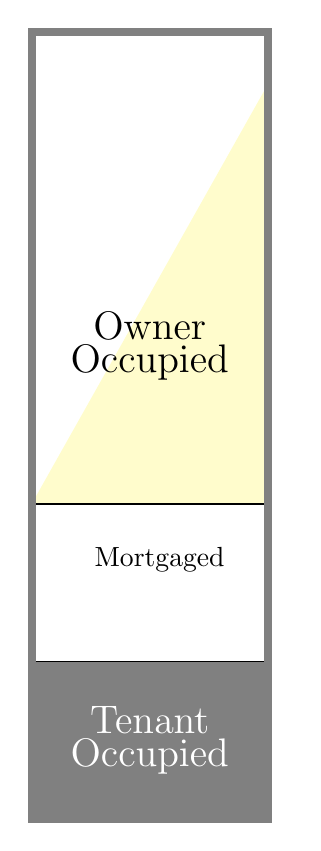
\begin{tikzpicture}{scale=.5}
%   \coordinate (planning) at (-5,1);%PREFACE
% \coordinate (economics) at (5,.75);%
%  \coordinate (geography) at (-.5,-2); %history
% \coordinate (finance) at (0,5); %  
\draw [fill=gray,] (0,0) rectangle (3,2); %TENANT


\draw [fill=yellow!20] (0,4)--(3,4)--(3,9.33); --cycle;% MORTGAGE %Calculation. 80\%owner, so  8 above the tenant line. 2/3*8=5.333. 5.333+2=



\draw[line width= 1mm, black!50] (0,0) rectangle (3,10);

\node at (1.5,6)
    [text width=2.4cm, align=center]
    {\baselineskip=20pt\Large Owner Occupied};
\node at (2,3.3)
    [text width=2.4cm]
    {\baselineskip=20pt Mortgaged};
\node at (1.5,1)
    [text width=2.4cm, align=center, white]
    {\baselineskip=20pt\Large Tenant Occupied};
\end{tikzpicture}
\end{center}

Figure: Housing Tenure 

The mortgage demonstrates the two aspects of financial instruments. It is both a financial instrument that enables  purchase and a financial asset that can be bought and sold. When we consider urban housing, it is the right to future income generated by capital, labour and the city itself through the agglomeration effects that drive productivity. It is an instrument that indirectly captures a share of the urban rents. As productivity rises, wages rise, rents rise, property prices rise and mortgages rise. 

For urban theory and policy formation it is important to distinguish between financial instruments that enable production of real assets, and instruments like  mortgages that primarily facilitate the transfer of real assets or rights to real estate  income. Housing developers borrow to purchase land for development and builders borrow to finance construction. While important, the financial instruments involved are not driving the financialization of housing.  The size of the loans involved is affected by the amount of land purchased and the potential rents earned by that land, but the degree of non-occupant ownership is not affected. *** CLARIFY
  
\begin{center}
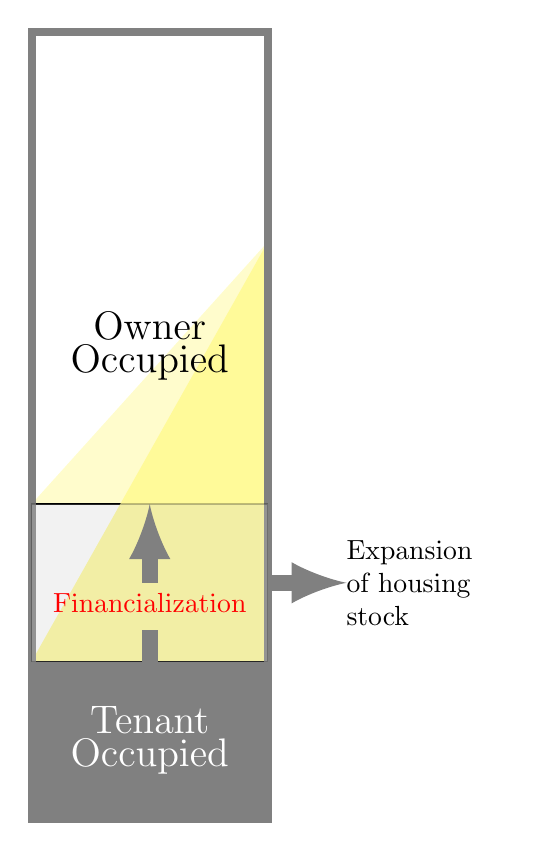
\begin{tikzpicture}{scale=.5}
\draw [fill=yellow!20] (0,4)--(3,4)--(3,7.33); --cycle;% MORTGAGE %Calculation. 80\%owner, so  8 above the tenant line. 2/3*8=5.333. 5.333+2=

\draw [fill=gray] (0,0) rectangle (3,2); %TENANT

\draw [fill=yellow!40] (0,2)--(3,2)--(3,7.33); --cycle;% MORTGAGE %Calculation. 80\%owner, so  8 above the tenant line. 2/3*8=5.333. 5.333+2=
\draw[line width= 1mm, black!50] (0,0) rectangle (3,10);

\node at (1.5,6)
    [text width=2.4cm, align=center]
    {\baselineskip=20pt\Large Owner Occupied};
%\node at (2,3.3)
    [text width=2.4cm]
    {\baselineskip=20pt Mortgaged};
    
\draw [fill=gray!40,opacity=.25] (0,2) rectangle (3,4); %fiancialization
\node at (1.5,1)
    [text width=2.4cm, align=center, white]
    {\baselineskip=20pt\Large Tenant Occupied};



\draw [gray,line width=2mm](1.5,2)--(1.5,2.4) node[above, red]{Financialization}; 
\draw [gray,-latex, line width=2mm](1.5,3)--(1.5,4);

\draw [gray,line width=2mm,-latex](3,3)--(4,3); \node at (5,3)[text width=2cm]{Expansion of housing stock}; 
\end{tikzpicture}
\end{center}

Figure: Financialization vs expansion of the housing stock 

\subsection{Investment trusts}

An example of a financial instrument designed specifically to support rent extraction and which  increases the degree of financialization of the housing supply is the  Real Estate Investment Trust (REIT).  A REIT is a company that owns, operates, or finances income-generating real estate and distribute the income to shareholders. There are other large owners of residential real estate such as life insurance companies and pension plans that behave similarly, but REITs are a relatively new financial instrument which is  expanding rapidly and attracting political attention for their effect on housing markets.  % REITs that develop new properties generally don't sell the properties they construct.

REITs have become increasingly popular in recent years.  An S\&P-Dow Jones research bulletin reported that over the  25 years to 2017, REITs outperformed stocks, bonds, and commodities. Because they have outperformed competing investments they have attracted  capital from other uses.

Developed in the USA  in 1960 (as an amendment to the Cigar Excise Tax Extension!) and in Canada in 1993, REITs are similar to mutual funds in making it possible for an individual, often small investors to earn dividends from real estate investments without having to buy, manage, or finance any properties themselves. There are questions about preferential tax treatment, and whether some REITs are really inappropriately sheltered real-estate corporations.  For the purpose of this thesis, they are simply one of the mechanisms for the financialization of housing.

They are not simply a neutral tool for saving however. According to a paper \cite{wangAnalyzeImpactREITs2021}\footnote{Guolin Wang. Analyze the Impact of REITs on the Irish Real Estate Market. Advances in Economics, Business and Management Research, volume 203, Proceedings of the 2021 3rd International Conference on Economic Management and Cultural Industry (ICEMCI 2021)} on REITS in the Irish housing market, ``REIT successfully reconnected the international financial market and the Irish real estate market.'' In other words, in Ireland, REITS have made it easier for international capital to buy Irish land. The entry of outside and footloose capital has had an effect on the resident population:  ``the large-scale acquisition of Irish real estate by REITs and other real estate buyers has also caused some new problems. First, the active management of assets by REITs and other investors has led to a rapid increase in rents''.\footnote{In IMF working paper WP/15/243 2015, Capital Account Liberalization and Inequality, Davide Furceri and Prakash Loungani found that for 149 countries from 1970 to 2010, ``after countries take steps to open their capital account, an increase in inequality in incomes within countries follows.'' The observation is consistent with our argument  that domestic rent-seeking in housing markets will increase inequality.}   \cite{furceriCapitalAccountLiberalization2015}

There is evidence that REITs affect real estate markets in other ways. A \href{https://www.ineteconomics.org/research/research-papers/the-role-of-public-reits-in-financialization-and-industry-restructuring}{report} from the Institute for New Economic Thinking, for example, argues that ``The evidence in this report shows that they are actually financial actors that aggressively buy up property assets and manage them to extract wealth at taxpayers’ expense. ''\footnote{The Role of Public REITs in Financialization and Industry Restructuring. Rosemary Batt and Eileen Appelbaum, with Tamar Katz* Working Paper No. 189 July 9th, 2022} ``\dots they have expanded the pool of capital available for transactions that monetize real property and turn it into tradable assets – financial widgets with little or no connection to the real purpose of the productive enterprises that occupy the properties they own.''

\subsection{Financialization and productivity}

When  a productive asset is acquired as a financial asset it remains productive. African land or land in Northern Ontario acquired by holding companies may even be made more productive. 
% the goal of such investments, however, is generally to achieve a capital gain over time. Financial analysis is essentially about rates of return on financial capital invested. The opportunity for capital gains  attracts financial capital to the housing market.%Financial managers have no interest is n in assets that are not expected to increase in value. 


% The financialization of urban housing benefits a globally distributed rentier class of urban landholders. We will make this more explicit below the incentive structure deriving the further financialization of the housing market.
